\documentclass[12pt, a4paper]{article}
\usepackage[utf8]{inputenc}
\usepackage[T2A]{fontenc}
\usepackage{indentfirst, setspace}
\usepackage{tabularx, multirow}
\usepackage[normalem]{ulem}
\usepackage[style=russian]{csquotes}
\usepackage[english,russian]{babel}
\usepackage{hyperref}
\usepackage{ragged2e}
\usepackage{caption}
\usepackage{wrapfig}
\usepackage{amsmath}
\usepackage{tikz}
\makeatletter
\def\@biblabel#1{#1. }
\makeatother
\captionsetup{labelsep=endash}
\usepackage{listings}
\linespread{1.3}
\lstset{
  language=C++,
  basicstyle=\ttfamily\small,
  keywordstyle=\color{blue},
  breaklines=true,
  commentstyle=\color{green},
  stringstyle=\color{red},
  extendedchars=\true,
  showstringspaces=false,
  keepspaces=true,
}

\usepackage[left=2cm,right=2cm,
    top=2cm,bottom=2cm,bindingoffset=0cm]{geometry}\begin{document}
\begin{titlepage}
     \fontsize{12}{12}\selectfont

  {\centering

   \begin{bf}

    \begin{wrapfigure}{l}{10mm}
        
\includegraphics[width=17mm]{photo_2023-12-14.jpeg}
    \end{wrapfigure}


    \noindent Министерство науки и высшего образования Российской Федерации

    \noindent Федеральное государственное бюджетное образовательное учреждение высшего образования

    \noindent \enquote{Московский государственный технический университет

     \noindent имени Н.Э. Баумана

     \noindent (национальный исследовательский университет)}

    \noindent (МГТУ им. Н.Э. Баумана)

   \end{bf}
  }

  \vspace{0.4cm}

  {\setstretch{0.1}
   \noindent\rule{\textwidth}{1mm}
   \noindent\rule{\textwidth}{0.5mm}

  }

  \fontsize{14}{21}\selectfont

  \noindent\begin{tabularx}{\textwidth}{l >{\centering\arraybackslash}X}
   ФАКУЛЬТЕТ & \flqq Фундаментальные Науки\frqq \\ \cline{2-2}

   КАФЕДРА & ФН-12 \flqq Математическое моделирование\frqq \\ \cline{2-2}
  \end{tabularx}

  \vspace{1cm}


  \begin{center}
   \begin{bf}

    \fontsize{24}{36}\selectfont
    ОТЧЕТ

    \fontsize{20}{30}\selectfont
    ПО ЛАБОРАТОРНОЙ РАБОТЕ НА ТЕМУ:

    Умножение матриц

   \end{bf}
  \end{center}

  \fontsize{14}{21}\selectfont
  \vspace{5cm}


  \noindent\begin{tabularx}{\textwidth}{ X >{\centering}p{4cm} p{1cm} c }
   Студент: & & & Мациевский И. М. \\ \cline{2-2} \cline{4-4}
   & \fontsize{10}{15}\selectfont дата, подпись & & \fontsize{10}{15}\selectfont Ф.И.О. \\
   Преподаватель: & & & Волкова Л. Л.\\ \cline{2-2} \cline{4-4}
   & \fontsize{10}{15}\selectfont дата, подпись & & \fontsize{10}{15}\selectfont Ф.И.О.
   \end{tabularx}

  \vspace{\fill}

  \begin{center}
   \it{Москва}, 2023
  \end{center}

  \thispagestyle{empty}
\end{titlepage}\newpage
\tableofcontents
\newpage
\section*{Введение}
\addcontentsline{toc}{section}{Введение}
\justifying
\textbf{Цель лабораторной работы}: провести сравнительный анализ алгоритмов умножения матриц.

Для достижения поставленной цели требуется решить следующие \textbf{задачи}.
\begin{enumerate}
\item Описать три алгоритма умножения матриц --- классический, Винограда и 
Штрассена.
\item Реализовать разработанные алгоритмы.
\item Выполнить тестирование реализации разработанных алгоритмов.
\item Дать оценку сложности алгоритмов.
\item Оценить эффективность каждого алгоритма (по памяти и времени).
\end{enumerate}
\newpage
\section{Аналитическая часть}
\textbf{Матрица ---} упорядоченный математический 
объект, обычно записываемый в виде прямоугольной 
таблицы элементов кольца/поля или другой структуры. 
Количество строк и столбцов задает размер этой 
матрицы. С матрицами можно производить различные 
действия, такие как транспонирование, сложение, 
умножения и др. 

\newpage
\section{Конструкторская часть}
\subsection{Классический алгоритм умножения матриц}
Пусть у нас есть две матрицы $A$ размерности $m \times n$ и $B$ 
размерности $n \times p$. Результирующая матрица будет иметь размерность $
m \times p$, и её элементы $C$ будут вычисляться следующим образом:

$C(i, k) = \sum_{j=1}^{n} A(i, j) \cdot B(j, k), \quad 1 \leq i \leq m, \quad 1 \leq k \leq p$.
\begin{enumerate}
    \item $A(i, j)$ - элемент матрицы $A$ в $i$-й строке и $j$-м столбце.
    \item $B(j, k)$ - элемент матрицы $B$ в $j$-й строке и $k$-м столбце.
    \item $C(i, k)$ - элемент результирующей матрицы $C$ в $i$-й строке и 
    $k$-м столбце.
\end{enumerate}
Этот процесс повторяется для всех $i$, $k$, что приводит к вычислению всех 
элементов матрицы $C$.
\subsection{Метод Штрассена}
Метод Штрассена представляет собой более эффективный алгоритм умножения матриц. 
Идея заключается в том, чтобы заменить обычные умножения матриц на более 
эффективные линейные комбинации элементов.\\
Для умножения двух матриц $A$ и $B$ размерности $n \times n$, метод Штрассена 
предлагает следующие рекуррентные формулы:
\[
\begin{aligned}
P_1 &= (A_{11} + A_{22}) \cdot (B_{11} + B_{22}), \\
P_2 &= (A_{21} + A_{22}) \cdot B_{11}, \\
P_3 &= A_{11} \cdot (B_{12} - B_{22}), \\
P_4 &= A_{22} \cdot (B_{21} - B_{11}), \\
P_5 &= (A_{11} + A_{12}) \cdot B_{22}, \\
P_6 &= (A_{21} - A_{11}) \cdot (B_{11} + B_{12}), \\
P_7 &= (A_{12} - A_{22}) \cdot (B_{21} + B_{22}),
\end{aligned}
\]
Результирующие блоки матрицы $C$:
\[
\begin{aligned}
C_{11} &= P_1 + P_4 - P_5 + P_7, \\
C_{12} &= P_3 + P_5, \\
C_{21} &= P_2 + P_4, \\
C_{22} &= P_1 - P_2 + P_3 + P_6.
\end{aligned}
\]

Таким образом, результат умножения матриц $A$ и $B$ получается из линейных 
комбинаций блоков $P_1, P_2, \ldots, P_7$.
\subsection{Метод Винограда}
Алгоритм Винограда включает следующие шаги.
\begin{enumerate}
    \item Создать новую матрицу $C$ размерностью $m \times n$ и заполните ее нулями.
    \item Создать вспомогательные массивы $row\_factor$ и $col\_factor$ для оптимизации вычислений. Их размерность равна числу строк матрицы $A$ и числу столбцов матрицы $B$ соответственно.
    \item Вычислить $row\_factor[i]$ как сумму произведений пар элементов из $A[i]$, умноженных на соответствующие элементы из $A[i]$.
    \item Вычислите $col\_factor[j]$ как сумму произведений пар элементов из $B[j]$, умноженных на соответствующие элементы из $B[j]$.
    \item Используя предварительно вычисленные $row\_factor$ и $col\_factor$, вычислите каждый элемент матрицы $C$ следующим образом: 
    \[ C[i][j] = rc\_f + \sum_{k=0}^{k-1} (A[i][k] + B[k][j]) \cdot (A[i][k+1] + B[k+1][j]) \text{, где}\]  \[ rc\_f = -row\_factor[i] - col\_factor[j] \] 
    \item Если размерность матрицы нечетна, нужно добавить к соответствующему элементу $C$ произведение соответствующих элементов из $A$ и $B$, которые не участвовали в основных вычислениях.
\end{enumerate}
\subsection{Функции программы}
Требуется разработать следующие функции.
\begin{itemize}
    \item[---] Функция ``matrixSum'' --- функция, которая складывает матрицы.
    \item[---] Функция ``matrixMultiplication'' --- функция, которая перемножает две матрицы.
    \item[---] Функция ``strassenMatrixMultiply'' --- функция для умножения матриц методом Штрассена.
    \item[---] Функция ``classicMatrixMultiply'' --- функция для умножения матриц классическим способом.
    \item[---] Функция ``matrixMultiplyVinograd'' ---  Функция для умножения матриц с использованием алгоритма Винограда.
    \item[---] Функция ``showMatrix'' --- функция для вывода матрицы.
\end{itemize}
\newpage
\section{Технологическая часть}
Для реализации выбран язык C++.
На листинге 1 представлена реализация программы
(Реализация~\ref{lst:label1})
\begin{lstlisting}[caption={Исходный код}, label={lst:label1}]
#include <iostream>
#include <vector>
#include <ctime>

using namespace std;

// Функция для сложения матриц
vector<vector<int>> matrixSum(const vector<vector<int>>& A, const vector<vector<int>>& B) {
    int n = A.size();
    vector<vector<int>> result(n, vector<int>(n, 0));

    for (int i = 0; i < n; i++) {
        for (int j = 0; j < n; j++) {
            result[i][j] = A[i][j] + B[i][j];
        }
    }

    return result;
}

// Функция для вычитания матриц
vector<vector<int>> matrixMultiplication(const vector<vector<int>>& A, const vector<vector<int>>& B) {
    int n = A.size();
    vector<vector<int>> result(n, vector<int>(n, 0));
    for (int i = 0; i < n; i++) {
        for (int j = 0; j < n; j++) {
            result[i][j] = A[i][j] - B[i][j];
        }
    }

    return result;
}

// Функция для умножения матриц методом Штрассена
vector<vector<int>> strassenMatrixMultiply(const vector<vector<int>>& A, const vector<vector<int>>& B) {
    int n = A.size();

    if (n <= 2) {
        vector<vector<int>> result(n, vector<int>(n, 0));
        for (int i = 0; i < n; i++) {
            for (int j = 0; j < n; j++) {
                for (int k = 0; k < n; k++) {
                    result[i][j] += A[i][k] * B[k][j];
                }
            }
        }

        return result;
    }

    int newSize = n;
    if (n % 2 != 0) {
        newSize++;
    }

    vector<vector<int>> newA(newSize, vector<int>(newSize, 0));
    vector<vector<int>> newB(newSize, vector<int>(newSize, 0));
    for (int i = 0; i < n; i++) {
        for (int j = 0; j < n; j++) {
            newA[i][j] = A[i][j];
            newB[i][j] = B[i][j];
        }
    }

    vector<vector<int>> A11(newSize / 2, vector<int>(newSize / 2, 0));
    vector<vector<int>> A12(newSize / 2, vector<int>(newSize / 2, 0));
    vector<vector<int>> A21(newSize / 2, vector<int>(newSize / 2, 0));
    vector<vector<int>> A22(newSize / 2, vector<int>(newSize / 2, 0));
    vector<vector<int>> B11(newSize / 2, vector<int>(newSize / 2, 0));
    vector<vector<int>> B12(newSize / 2, vector<int>(newSize / 2, 0));
    vector<vector<int>> B21(newSize / 2, vector<int>(newSize / 2, 0));
    vector<vector<int>> B22(newSize / 2, vector<int>(newSize / 2, 0));
    for (int i = 0; i < newSize / 2; i++) {
        for (int j = 0; j < newSize / 2; j++) {
            A11[i][j] = newA[i][j];
            A12[i][j] = newA[i][j + newSize / 2];
            A21[i][j] = newA[i + newSize / 2][j];
            A22[i][j] = newA[i + newSize / 2][j + newSize / 2];

            B11[i][j] = newB[i][j];
            B12[i][j] = newB[i][j + newSize / 2];
            B21[i][j] = newB[i + newSize / 2][j];
            B22[i][j] = newB[i + newSize / 2][j + newSize / 2];
        }
    }

    vector<vector<int>> M1 = strassenMatrixMultiply(matrixSum(A11, A22), matrixSum(B11, B22));
    vector<vector<int>> M2 = strassenMatrixMultiply(matrixSum(A21, A22), B11);
    vector<vector<int>> M3 = strassenMatrixMultiply(A11, matrixMultiplication(B12, B22));
    vector<vector<int>> M4 = strassenMatrixMultiply(A22, matrixMultiplication(B21, B11));
    vector<vector<int>> M5 = strassenMatrixMultiply(matrixSum(A11, A12), B22);
    vector<vector<int>> M6 = strassenMatrixMultiply(matrixMultiplication(A21, A11), matrixSum(B11, B12));
    vector<vector<int>> M7 = strassenMatrixMultiply(matrixMultiplication(A12, A22), matrixSum(B21, B22));

    vector<vector<int>> C11 = matrixSum(matrixMultiplication(matrixSum(M1, M4), M5), M7);
    vector<vector<int>> C12 = matrixSum(M3, M5);
    vector<vector<int>> C21 = matrixSum(M2, M4);
    vector<vector<int>> C22 = matrixSum(matrixSum(matrixMultiplication(M1, M2), M3), M6);

    vector<vector<int>> result(newSize, vector<int>(newSize));
    for (int i = 0; i < newSize / 2; i++) {
        for (int j = 0; j < newSize / 2; j++) {
            result[i][j] = C11[i][j];
            result[i][j + newSize / 2] = C12[i][j];
            result[i + newSize / 2][j] = C21[i][j];
            result[i + newSize / 2][j + newSize / 2] = C22[i][j];
        }
    }

    // Матрица без лишних нулей
    vector<vector<int>> finalResult(n, vector<int>(n));
    for (int i = 0; i < n; i++) {
        for (int j = 0; j < n; j++) {
            finalResult[i][j] = result[i][j];
        }
    }

    return finalResult;
}

// Функция для умножения матриц классическим способом
vector<vector<int>> classicMatrixMultiply(const vector<vector<int>>& matA, const vector<vector<int>>& matB) {

    if (matA[0].size() != matB.size()) {
        cout << "Невозможно умножить матрицы: неподходящие размеры" << endl;
        return {};
    }

    vector<vector<int>> result(matA.size(), vector<int>(matB[0].size(), 0));

    for (int i = 0; i < matA.size(); i++) {
        for (int j = 0; j < matB[0].size(); j++) {
            for (int k = 0; k < matA[0].size(); k++) {
                result[i][j] += matA[i][k] * matB[k][j];
            }
        }
    }

    return result;
}

// Функция для умножения матриц с использованием алгоритма Винограда
vector<vector<int>> matrixMultiplyVinograd(const vector<vector<int>>& matA, const vector<vector<int>>& matB) {
    int rowsA = matA.size();
    int colsA = matA[0].size();
    int rowsB = matB.size();
    int colsB = matB[0].size();

    if (colsA != rowsB) {
        cout << "Невозможно умножить матрицы: неподходящие размеры" << endl;
        return {};
    }

    vector<vector<int>> result(rowsA, vector<int>(colsB, 0));

    // Предварительные вычисления для оптимизации
    vector<int> rowFactor(rowsA, 0);
    vector<int> colFactor(colsB, 0);
    for (int i = 0; i < rowsA; i++) {
        for (int k = 0; k < colsA - 1; k += 2) {
            rowFactor[i] += matA[i][k] * matA[i][k + 1];
        }
    }
    for (int j = 0; j < colsB; j++) {
        for (int k = 0; k < rowsB - 1; k += 2) {
            colFactor[j] += matB[k][j] * matB[k + 1][j];
        }
    }

    // Основной цикл умножения с использованием предварительных вычислений
    for (int i = 0; i < rowsA; i++) {
        for (int j = 0; j < colsB; j++) {
            result[i][j] = -rowFactor[i] - colFactor[j];
            for (int k = 0; k < colsA - 1; k += 2) {
                result[i][j] += (matA[i][k] + matB[k + 1][j]) * (matA[i][k + 1] + matB[k][j]);
            }
            if (colsA % 2 != 0) {
                result[i][j] += matA[i][colsA - 1] * matB[rowsB - 1][j];
            }
        }
    }

    return result;
}

// Функция для вывода матрицы
void showMatrix(const vector<vector<int>>& mat) {
    for (const auto& row : mat) {
        for (int val : row) {
            cout << val << " ";
        }
        cout << endl;
    }
}

int main(){
    setlocale(0, "");
    cout << "Каким методом Вы хотите перемножить матрицы?" << endl;
    cout << "Классический метод - 1" << endl;
    cout << "Метод Винограда - 2" << endl;
    cout << "Метод Штрассена - 3" << endl;
    int choose = 0;
    double medtime = 0;
    cin >> choose;
    
    if (choose == 1) {
        
        vector<vector<int>> matrixA = { {1, 2, 3}, {4, 5, 6}, {7, 8, 9} };
        vector<vector<int>> matrixB = { {9, 8, 7}, {6, 5, 4}, {3, 2, 1} };
        
        cout << "Матрица A:" << endl;
        showMatrix(matrixA);
        cout << endl;
        
        cout << "Матрица B:" << endl;
        showMatrix(matrixB);
        cout << endl;
        
        clock_t start_time = clock();
        vector<vector<int>> result = classicMatrixMultiply(matrixA, matrixB);
        clock_t end_time = clock();
        double cpu_time = (double(end_time - start_time)) / CLOCKS_PER_SEC;
        medtime += cpu_time;
        cout << "Результат умножения классическим методом:" << endl;
        showMatrix(result);
        cout << "Процессорное время: " << cpu_time << endl;
        cout << endl;
    }
    else if (choose == 2) {
        
        vector<vector<int>> matrixA = { {1, 2, 3}, {4, 5, 6}, {7, 8, 9} };
        vector<vector<int>> matrixB = { {9, 8, 7}, {6, 5, 4}, {3, 2, 1} };
        
        cout << "Матрица A:" << endl;
        showMatrix(matrixA);
        cout << endl;
        
        cout << "Матрица B:" << endl;
        showMatrix(matrixB);
        cout << endl;
        
        clock_t start_time = clock();
        vector<vector<int>> result = matrixMultiplyVinograd(matrixA, matrixB);
        clock_t end_time = clock();
        double cpu_time = (double(end_time - start_time)) / CLOCKS_PER_SEC;
        medtime += cpu_time;
        cout << "Результат умножения с помощью алгоритма Винограда:" << endl;
        showMatrix(result);
        cout << "Процессорное время: " << cpu_time << endl;
        cout << endl;
    }
    else if (choose == 3) {
        vector<vector<int>> matrixA = { {1, 2, 3}, {4, 5, 6}, {7, 8, 9} };
        vector<vector<int>> matrixB = { {9, 8, 7}, {6, 5, 4}, {3, 2, 1} };
        cout << "Матрица A:" << endl;
        showMatrix(matrixA);
        cout << endl;
        cout << "Матрица B:" << endl;
        showMatrix(matrixB);
        cout << endl;
        
        clock_t start_time = clock();
        vector<vector<int>> result = strassenMatrixMultiply(matrixA, matrixB);
        clock_t end_time = clock();
        double cpu_time = (double(end_time - start_time)) / CLOCKS_PER_SEC;
        medtime += cpu_time;
        cout << "Результат умножения с помощью алгоритма Штрассена:" << endl;
        showMatrix(result);
        cout << "Процессорное время: " << cpu_time << endl;
        cout << endl;
    }
    else {
        cout << "Неверный выбор" << endl;
    }
    return 0;
}
\end{lstlisting}
\newpage
\begin{center}
	\textbf{Примеры работы}
\end{center}
На рисунках 1---7 представлены примеры работы описаннных выше алгоритмов.
\begin{enumerate}
	\item На вход подаются две матрицы размерности $3 \times 3$, 
	программа выводит их произведение, рассчитанное по классическому алгоритму.
	Результат приведён на рис.~\ref{img:grap1}.
	\begin{figure}[h]
  		\center{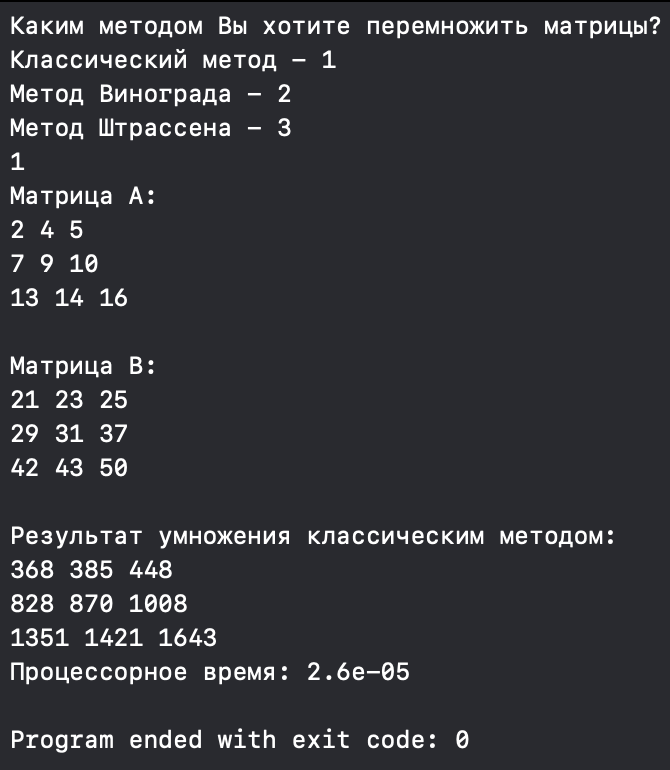
\includegraphics[scale=0.6]{ex1.png}}
  		\caption{Пример работы 1}
  		\label{img:grap1}
	\end{figure}
	\item На вход подаются две матрицы размерности $3 \times 3$, 
	программа выводит их произведение, рассчитанное по методу Винограда.
	Результат приведён на рис.~\ref{img:grap2}.
	\begin{figure}[h]
  		\center{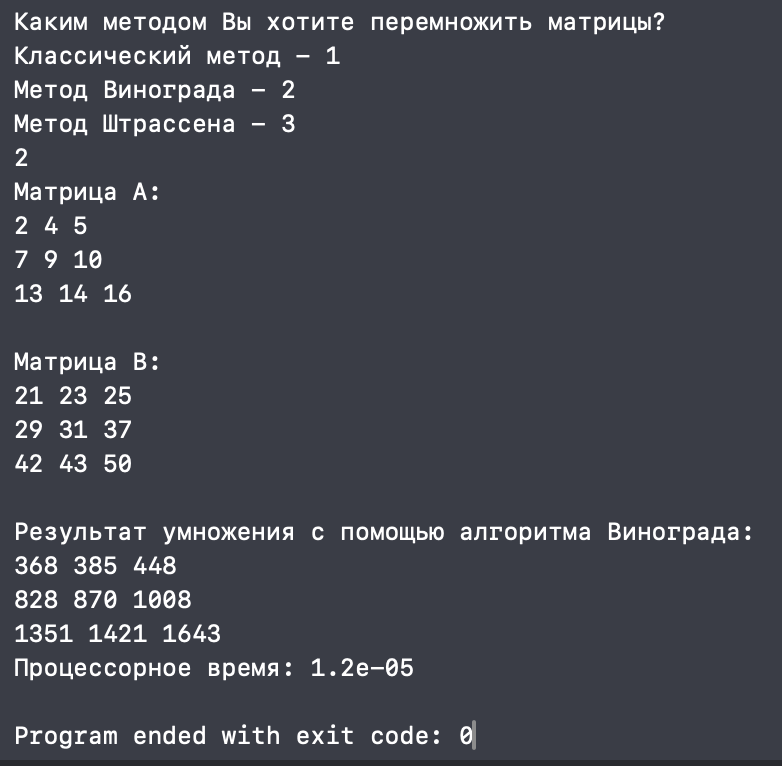
\includegraphics[scale=0.6]{ex2.png}}
  		\caption{Пример работы 2}
  		\label{img:grap2}
	\end{figure}
	\newpage
	\item На вход подаются две матрицы размерности $3 \times 3$, 
	программа выводит их произведение, рассчитанное по методу Штрассена.
	Результат приведён на рис.~\ref{img:grap3}.	
	\begin{figure}[h]
  		\center{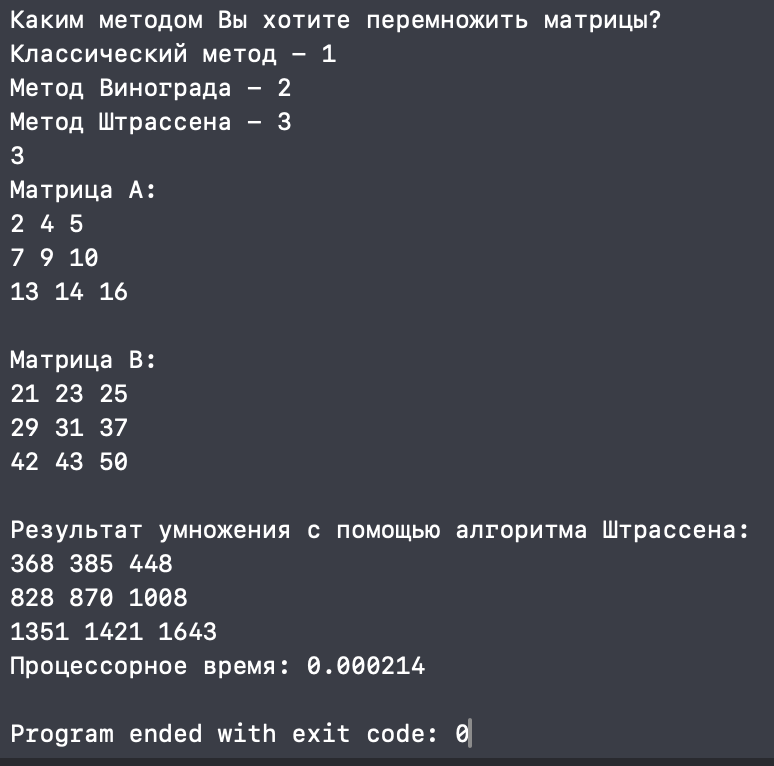
\includegraphics[scale=0.6]{ex3.png}}
  		\caption{Пример работы 3}
  		\label{img:grap3}
	\end{figure}
	\newpage
	\item На вход подаются две матрицы размерности $6 \times 6$, 
	программа выводит их произведение, рассчитанное по классическому алгоритму.
	Результат приведён на рис.~\ref{img:grap4}.
	\begin{figure}[h]
  		\center{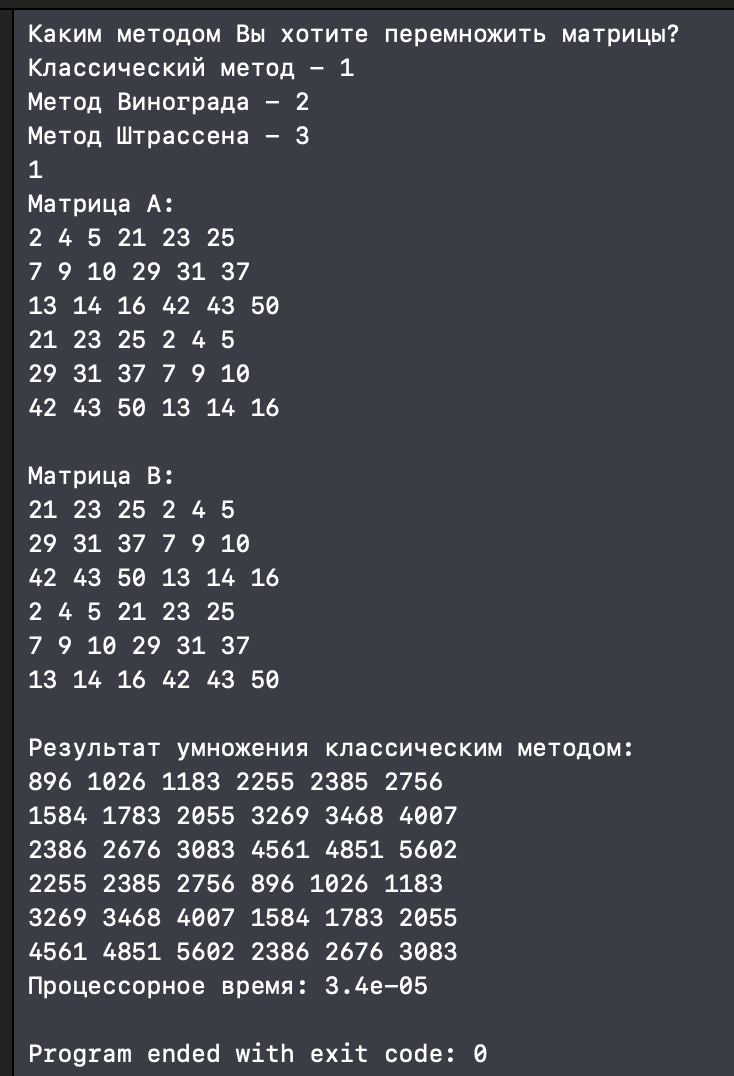
\includegraphics[scale=0.6]{ex4.png}}
  		\caption{Пример работы 4}
  		\label{img:grap4}
	\end{figure}
	\newpage
	\item На вход подаются две матрицы размерности $6 \times 6$, 
	программа выводит их произведение, рассчитанное по методу Винограда.
	Результат приведён на рис.~\ref{img:grap5}.	
	\begin{figure}[h]
  		\center{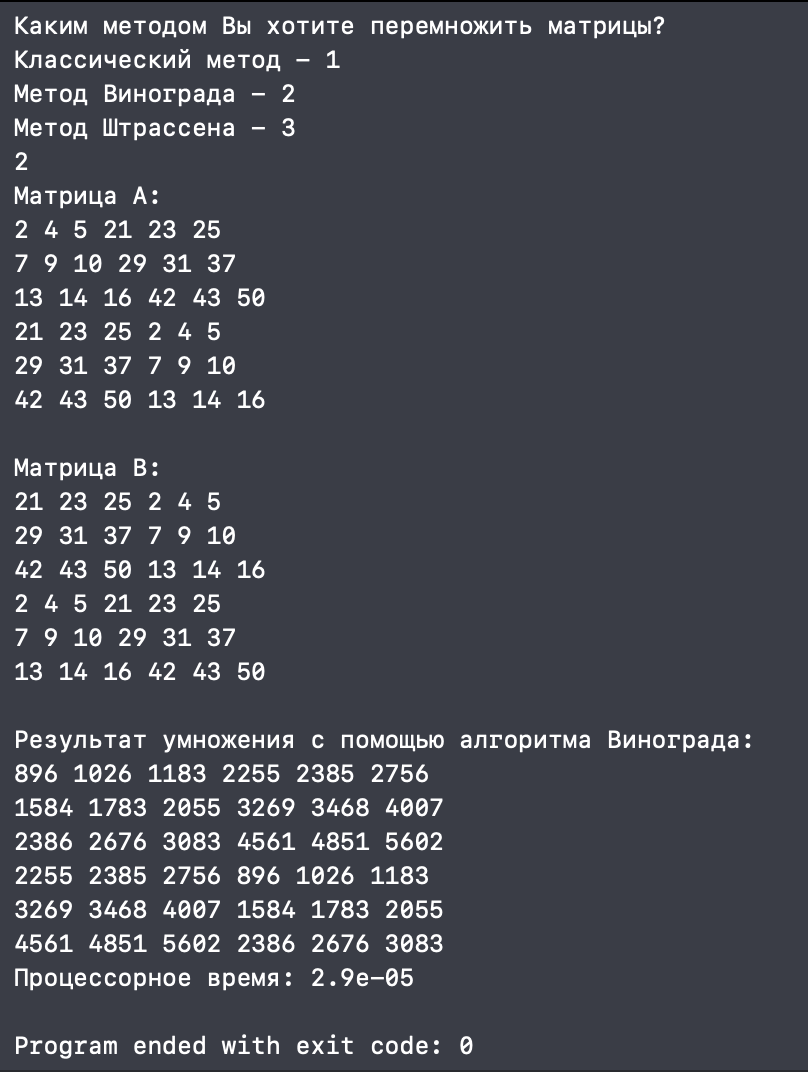
\includegraphics[scale=0.6]{ex5.png}}
  		\caption{Пример работы 5}
  		\label{img:grap5}
	\end{figure}
	\newpage
	\item На вход подаются две матрицы размерности $6 \times 6$, 
	программа выводит их произведение, рассчитанное по методу Штрассена.
	Результат приведён на рис.~\ref{img:grap6}.	
	\begin{figure}[h]
  		\center{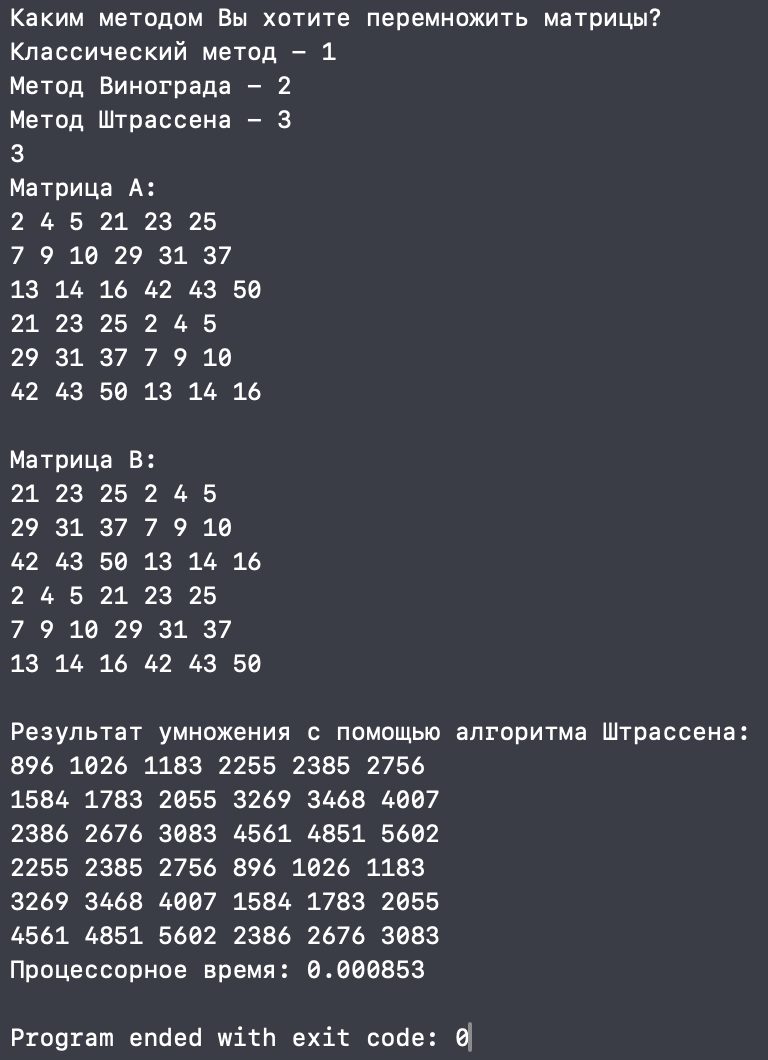
\includegraphics[scale=0.6]{ex6.png}}
  		\caption{Пример работы 6}
  		\label{img:grap6}
	\end{figure}
	\newpage
	\item На вход подаются две матрицы, одна размерности $6 \times 6$, другая 
	размерности $6 \times 3$, программа выводит ошибку.	
	Результат приведён на рис.~\ref{img:grap7}.
	\begin{figure}[h]
  		\center{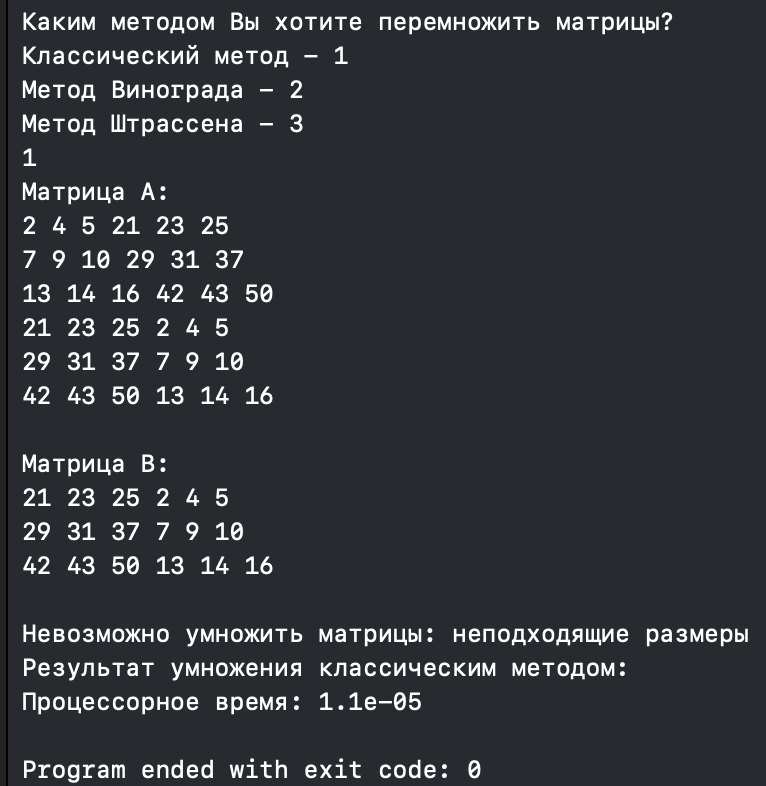
\includegraphics[scale=0.6]{ex7.png}}
  		\caption{Пример работы 7}
  		\label{img:grap7}
	\end{figure}
\end{enumerate}
\newpage
\section{Исследовательская часть}
\textbf {Анализ эффективности.}
Классический способ умножения матриц имеет временную сложность $O(n^3)$, где 
$n$ --- размерность матрицы. Это означает, что время выполнения операции 
умножения матриц линейно зависит от куба размера матрицы. Как результат, общее 
количество операций для умножения двух матриц размером $m \times p$ и $p \times 
n$ составляет $m \cdot p \cdot n$ умножений и $m \cdot n \cdot (p - 1)$ 
сложений.

Умножение матриц с помощью метода Винограда дает больший выигрыш во временной 
сложности. Она составяет $O(n^{2,3755})$, где $n$ --- размерность матрицы. 

Метод Штрассена умножает матрицы за время  $O(n^{\log _{2}7})=O(n^{2.81})$, что даёт выигрыш на больших плотных матрицах. Если обозначить количество операций умножения как $M(n)$, то для обычного метода умножения матриц размера $2^n \times 2^n$ имеем $M(n) = 8^n$. Алгоритм Штрассена снижает количество операций умножения до $M(n) = 7^n$, что означает уменьшение сложности. Он достигает этого за счет уменьшения числа стандартных умножений матриц.

\newpage
\section*{Заключение}
\addcontentsline{toc}{section}{Заключение}
Цель лабораторной работы достигнута. Проведён сравнительный анализ алгоритмов умножения матриц.

В результате выполнения лабораторной работы были выполнены все задачи.
\begin{enumerate}
\item Описаны три алгоритма умножения матриц --- классический, Винограда и Штрассена.
\item Реализованы разработанные алгоритмы.
\item Выполнено тестирование реализации разработанных алгоритмов.
\item Дана оценка сложности алгоритмов.
\item Оценена эффективность каждого алгоритма (по памяти и времени).
\end{enumerate}
\newpage
\begin{center}
\begin{thebibliography}{}
\addcontentsline{toc}{section}{Список используемых источников}
\bibitem{book}Т.Кормен, Ч.Лейзерсон, Р.Ривест, К.Штайн - Алгоритмы. Построение 
и анализ. Издание 3-е. Издательство: Диалектика, 2020 г. - 1328 c.
\end{thebibliography}
\end{center}
\end{document}